% assignment_4.tex
% CS 8735 - Unsupervised Learning (Fall 2015)
%     University of Missouri-Columbia
%             Chanmann Lim
%            November 2015

\documentclass[a4paper]{article}

\usepackage[margin=1 in]{geometry}
\usepackage{listings}
\usepackage{amsmath}
\usepackage{graphicx}
\usepackage{float}

\everymath{\displaystyle}
\DeclareMathOperator*{\argmax}{\arg\!\max}
\DeclareMathOperator*{\argmin}{\arg\!\min}

\begin{document}
\title{CS 8735: Report for assignment 4}
\author{Chanmann Lim}
\date{November 12, 2015}
\maketitle

\noindent The Matlab code for all experiments is in the \textbf{Appendix} section.

\paragraph{Problem 1.} In this task, we are going carry out spectral clustering on synthetic Circle.dat dataset. The first step in spectral clustering is to construct sparse graph by considering each data-point as a vertex of the Graph G(V,E) then connect two vertices that have the squared Euclidean distance smaller than $\epsilon = 1.5$. Creating an edge $e_{ij}$ when

\begin{equation}
	||x_i-x_j||^2 < \epsilon  \quad     \forall i,j
\end{equation}

Then using this sparse graph to generate n-by-n W matrix where n is the size of the dataset and $w(i, j)$ , the element at row $i^{th}$ and column $j^{th}$ is defined as

\begin{equation}
	w(i, j) = e^{\frac{-||x_i-x_j||^2}{\sigma^2}} \quad \text{if e\textsubscript{ij} exists and 0 otherwise}
\end{equation}

where $\sigma^2=2$, then we compute diagonal D matrix where each diagonal element Dii is the significance of each vertex:

\begin{equation}
	D_{ii}= \sum_{j\in V} w(i,j)
\end{equation}

Next, we define the graph Laplacian matrix $L = D – W$ and perform transformation on L to get normalized graph Laplacian matrix $\tilde{L}=D^{-1/2} LD^{-1/2}$ finally we can carry out eigen analysis on the normalized graph Laplacian matrix to obtain the eigenvalues and eigenvectors for our clustering task.

\paragraph{a)} The smallest five eigenvalues we got are [0, 0.0002, 0.0024, 0.0083, 0.0158].
\paragraph{b)} In minimizing the normalized cut spectral clustering pushes the smallest eigenvalue to zero hence it is no longer be appropriate for clustering task and we have to use the eigenvector $z_1$ that corresponding to the first non-zero eigenvalue to compute $y_1=D^{-1/2} z_1$ then assign $x_i$ to cluster C1 if $y_i < median (y)$ otherwise assign $x_i$ to cluster C2.

  \begin{figure}[H]
    \centering
      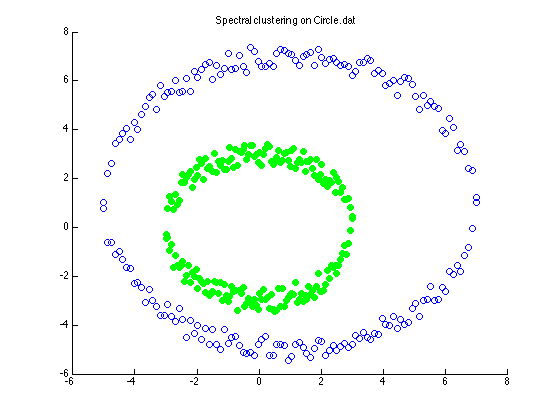
\includegraphics[scale=.47]{images/1.png}
    \caption{Plot of cluster assignment}
  \end{figure}

\paragraph{Problem 2.} In language modeling training, given four commands and a list of eight words we are going carry out latent semantic analysis by employing singular value decomposition (SVD) to transform the W (word by document) matrix into a smooth representation or concept of document namely "scaled document vectors" then we are going to merge a new test document and project its scaled document vector by mean of "fold-in" method and finally to compute the Euclidean distance between the new test command and the existing commands then rank them accordingly.

\paragraph{a)} $W_{8\times4}$ matrix is constructed such that its element $W_{ij} = (1-\epsilon_i)\frac{C_{ij}}{n_j}$ where $C_{ij}$ is the numbers of $word_i$ occurred in $document_j$, $n_j$ is the numbers of words in $document_j$ and $\epsilon_i$ is the normalized entropy of $word_i$ in the training set.

\begin{align}
	\epsilon_i &= \frac{-\sum_{j=1}^N \frac{C_{ij}}{t_i} \log \frac{C_{ij}}{t_i}}{-\sum_{j=1}^N \frac{1}{N} \log \frac{1}{N}} \\
		&= -\frac{1}{\log N} \sum_{j=1}^N \frac{C_{ij}}{t_i} \log \frac{C_{ij}}{t_i}
\end{align}

and $t_i = \sum_{j=1}^N C_{ij}$ with log being log base 2 when computing $\epsilon_i$. We obtain:

\begin{equation}
	W = \begin{bmatrix}
            0.0519  &  0.0519  &  0.0415   &      0 \\
		    0.0519  &  0.0519  &  0.0415   &      0 \\
	        0       &  0       &  0        & 0 \\
			0.1250  &       0  &  0.1000   &      0 \\
			0   & 0.2500   &     0         & 0 \\
			0   &      0   & 0.1000  &  0.1667 \\
			0   &      0   &     0   & 0.3333 \\
			0   &      0   &     0   &      0
        \end{bmatrix}
\end{equation}

\paragraph{b)} Next we decompose W by carry out SVD decomposition $W = U_RS_RV_R^T$ and we obtain:

\begin{equation}
	U_R = \begin{bmatrix}
			0.0200 &  -0.2450  &  0.2798 &   0.1085 \\
			0.0200 &  -0.2450  &  0.2798 &   0.1085 \\
			0.0000 &   0.0000  & -0.0000 &   0.0000 \\
			0.0449 &  -0.1263  &  0.8121 &   0.2857 \\
			0.0066 &  -0.9280  & -0.2760 &  -0.0484 \\
			0.4768 &  -0.0313  &  0.2636 &  -0.8380 \\
			0.8774 &   0.0416  & -0.1955 &   0.4362 \\
			0      &   0       &  0      &   0
		\end{bmatrix}
\end{equation}

\begin{equation}
	S_R = \begin{bmatrix}
			 0.3759   &      0    &     0    &     0 \\
		     0  &  0.2633   &      0  &       0 \\
		     0  &       0   & 0.1903  &       0 \\
		     0  &       0   &      0  &  0.0662
		\end{bmatrix}
\end{equation}

\begin{equation}
	V_R = \begin{bmatrix}
			0.0204 &  -0.1565 &   0.6862  &  0.7101 \\
			0.0099 &  -0.9776 &  -0.2100  & -0.0128 \\
			0.1432 &  -0.1371 &   0.6875  & -0.6986 \\
			0.9894 &   0.0329 &  -0.1116  & 0.0866
		\end{bmatrix}
\end{equation}
	
\paragraph{c)} By keeping the eigenvectors corresponding to the largest tow eigenvalues and computing the scaled document vectors of the four documents with $\bar{V}=S_RV_R^T$ we obtain dimension reduction in document smooth representation.

\begin{equation}
	\bar{V_2} = \begin{bmatrix}
			0.0077  &  0.0037  &  0.0538  &  0.3719 \\
			-0.0412 &  -0.2574 &  -0.0361 &   0.0087
		\end{bmatrix}
\end{equation}

\paragraph{d)} For the new test document we use "fold-in" method to compute $\bar{v_2}(5) = U_{8\times 2}^T \tilde{d_5}$ where $\tilde{d_5} = (1-\epsilon_i)\frac{C_{i5}}{n_5}$ and we obtain:

\begin{equation}
	\bar{v_2}(5) = \begin{bmatrix}
			    0.0606 \\
			   -0.0166
		\end{bmatrix}
\end{equation}

\paragraph{e)} Finally we compute the Euclidean distance between the test command (d-5) and the training commands using their scaled document vector.

\begin{center}
    \begin{tabular}{ |c |c |c |c |c | }
      \hline
       & d-1 & d-2 & d-3 & d-4 \\ \hline
      d-5 &     0.0584  &  0.2474  &  0.0206 &   0.3123 \\ \hline
    \end{tabular}
\end{center}

Hence the closest neighbors of d-5 rank from d-3, d-1, d-2 and d-4 sequentially.

  \begin{figure}[H]
    \centering
      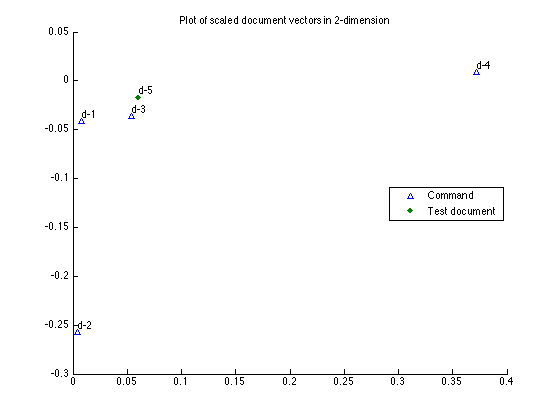
\includegraphics[scale=.57]{images/doc_vecs.png}
    \caption{Plot of scaled document vector in 2-dimension}
  \end{figure}

\newpage
\subsection*{Appendix:}
	\lstinputlisting[language=Matlab, title=\lstname, basicstyle=\footnotesize]{assignment_4.m}
	\lstinputlisting[language=Matlab, title=\lstname, basicstyle=\footnotesize]{problem_1.m}
	\lstinputlisting[language=Matlab, title=\lstname, basicstyle=\footnotesize]{problem_2.m}
	\lstinputlisting[language=Matlab, title=\lstname, basicstyle=\footnotesize]{problem_3.m}
	\lstinputlisting[language=Matlab, title=\lstname, basicstyle=\footnotesize]{problem_4.m}
	\lstinputlisting[language=Matlab, title=\lstname, basicstyle=\footnotesize]{problem_1.m}
	\lstinputlisting[language=Matlab, title=\lstname, basicstyle=\footnotesize]{Prob.m}
	\lstinputlisting[language=Matlab, title=\lstname, basicstyle=\footnotesize]{entropy.m}
\end{document}